
% \begin{figure}[h]
%     \centering
%     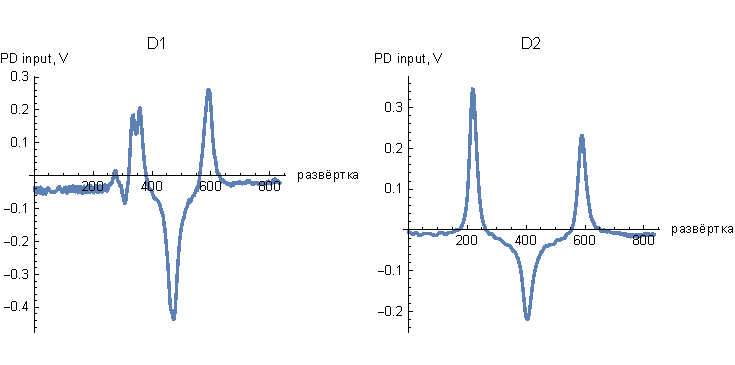
\includegraphics[width=0.8\textwidth]{D:\\Kami\\git_folder\\notes_5sem\\rqc\\data_processing_1\\D12.pdf}
%     \caption{Разность сигналов с насыщающем пучком и без для линий D${}_1$ и D${}_2$}
%     \label{fig:exp1}
% \end{figure}


\begin{figure}[h]
    \centering
    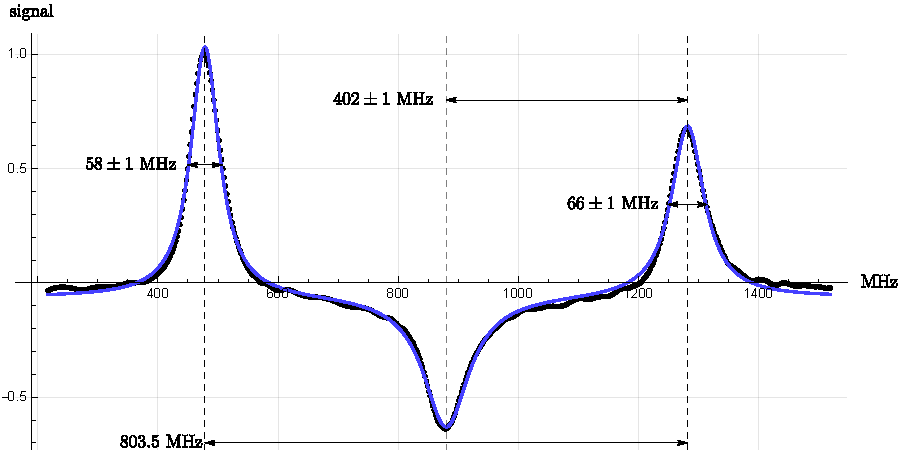
\includegraphics[width=0.7\textwidth]{D:\\Kami\\git_folder\\notes_5sem\\rqc\\data_processing_1\\exp_D2.pdf}
    \caption{Полученное уширение линий для D2}
    \label{fig:expD2}
\end{figure}


\begin{figure}[h]
    \centering
    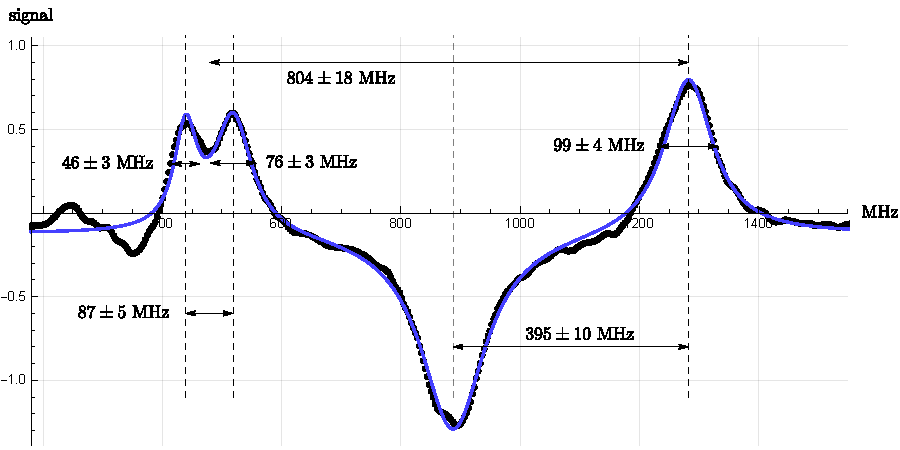
\includegraphics[width=0.7\textwidth]{D:\\Kami\\git_folder\\notes_5sem\\rqc\\data_processing_1\\exp_D1.pdf}
    \caption{Полученное уширение линий для D1}
    \label{fig:expD1}
\end{figure}


\begin{figure}[h!]
    \centering
    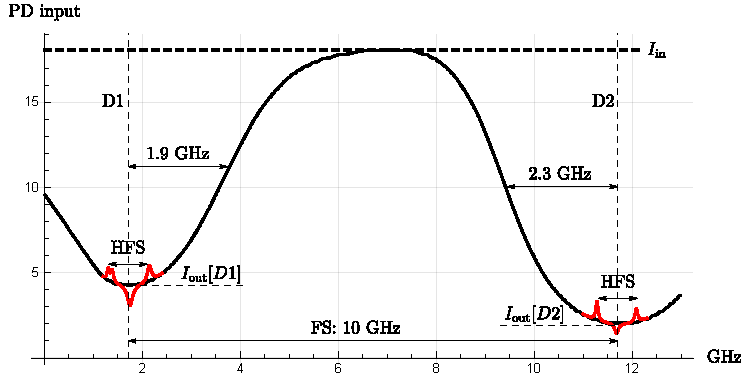
\includegraphics[width=0.7\textwidth]{D:\\Kami\\git_folder\\notes_5sem\\rqc\\data_processing_1\\exp_D12_v2.pdf}
    \caption{Полученное уширение линий для D1 и D2}
    \label{fig:expD12}
\end{figure}


\begin{figure}[ht]
    \centering
    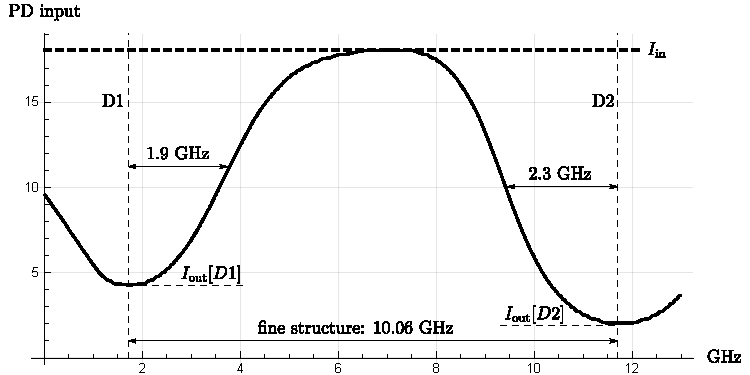
\includegraphics[width=0.7\textwidth]{D:\\Kami\\git_folder\\notes_5sem\\rqc\\data_processing_1\\exp_D12_v1.pdf}
    \caption{Полученное уширение линий для D1 и D2}
    \label{fig:expD12}
\end{figure}